\documentclass[journal]{IEEEtran}

\usepackage{cite}
%\usepackage{algorithmic}
\usepackage{fixltx2e}
\usepackage{url}
\usepackage{graphicx}
\usepackage{float}
\usepackage{amsmath}
\usepackage[]{algorithm2e}



\floatstyle{ruled}
\newfloat{program}{h}{lop}
\floatname{program}{Code}


%\pagestyle{empty}
\usepackage[latin1]{inputenc}
\usepackage{subfig}


%-------------------------------------------------------------------------
% Use a small font for the verbatim environment
\makeatletter  % makes '@' an ordinary character
\renewcommand{\verbatim@font}{
  \ttfamily\footnotesize\itshape\catcode`\<=\active\catcode`\>=\active }
\makeatother % makes '@' a special symbol again
%-------------------------------------------------------------------------
%

\frenchspacing

\sloppy

\pagestyle{empty}


% correct bad hyphenation here
\hyphenation{op-tical net-works semi-conduc-tor}


\begin{document}


\title{Multimedia Big Data Computing with Spark on MareNostrum Supercomputer}

% author names and IEEE memberships
% note positions of commas and nonbreaking spaces ( ~ ) LaTeX will not break
% a structure at a ~ so this keeps an author's name from being broken across
% two lines.
% use \thanks{} to gain access to the first footnote area
% a separate \thanks must be used for each paragraph as LaTeX2e's \thanks
% was not built to handle multiple paragraphs
%

%\author{
%        Ruben~Tous,	
%	Jordi~Torres,
%	Eduard Ayguad\'e
%                       
%\thanks{Ruben Tous, Jordi Torres and Eduard Ayguad\'e are with the Barcelona Supercomputing Center (BSC) and the Universitat Polit\`ecnica de Catalunya - BarcelonaTech (UPC), Barcelona, Spain}
%}

\author{
        Ruben~Tous,  
	Jordi~Torres and
	Eduard~Ayguad\'e
	
                       
\thanks{Ruben Tous, Jordi Torres and Eduard Ayguadé are with the Barcelona Supercomputing Center (BSC) and the Universitat Polit\`ecnica de Catalunya - BarcelonaTech (UPC), Barcelona, Spain}
}


% The paper headers
%\markboth{IEEE Multimedia,~Vol.~X, No.~X, Month~2008}%
%{Shell \MakeLowercase{\textit{et al.}}: Bare Demo of IEEEtran.cls for Journals}
% The only time the second header will appear is for the odd numbered pages
% after the title page when using the twoside option.
%
% *** Note that you probably will NOT want to include the author's ***
% *** name in the headers of peer review papers.                   ***
% You can use \ifCLASSOPTIONpeerreview for conditional compilation here if
% you desire.


% make the title area
\maketitle\thispagestyle{empty}


\begin{abstract}
In this paper we describe the design and evaluation of a framework to enable multimedia Spark workloads on MareNostrum, a petascale supercomputer. As far as we know, this is the first attempt to investigate optimized deployment configurations of this kinkd of workloads on a petascale HPC setup. We present the design of the framework and evaluate the scalability of the system. We examine the impact of different configurations including parallelism, storage and networking alternatives, and we discuss several aspects in executing multimedia big data workloads on a computing system that is based on the compute-centric paradigm. We derive conclusions to facilitate systematic and optimized methodologies for fine-tuning this kind of applications on large clusters. 
\end{abstract}


% Note that keywords are not normally used for peerreview papers.
%\begin{IEEEkeywords}
%TODO
%\end{IEEEkeywords}





\section{Introduction}

\IEEEPARstart{N}{}
owadays, there is a growing interest in exploiting the photos that users share on social networks such as Instagram or Twitter \cite{doi:10.1108/JRIM-07-2015-0047}\cite{conf/bigdataconf/Tous16}

TODO (Ruben + help from Mouna)

\section{Related Work}
\label{sec:rw}

TODO (Ruben + help from Mouna)

\section{A framework to enable multimedia big data workloads on MareNostrum, an HPC setup}
\label{sec:spark4mn}

TODO (Ruben)

\section{Benchmarking applications}
\label{sec:exps1}

\subsection{Bag-of-Words based image classification on Instagram}

TODO (Mouna)

TODO (Mouna)

\begin{figure}
\centering
\subfloat{
\includegraphics[width=0.9in, height=0.9in]{img/spam1} \label{fig:ob_inflamatory_histology}}
\subfloat{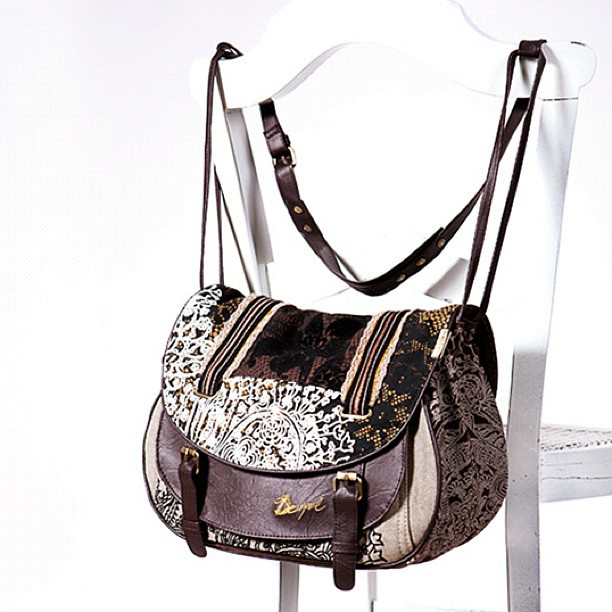
\includegraphics[width=0.9in, height=0.9in]{img/spam2} \label{fig:ob_inflamatory_histology}}
\subfloat{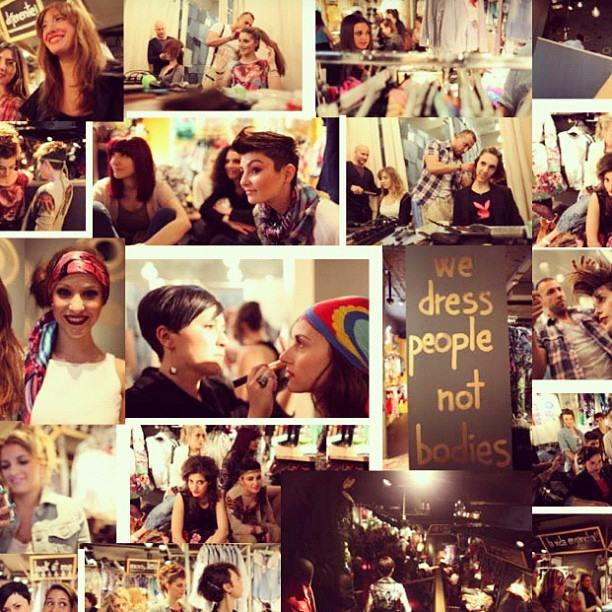
\includegraphics[width=0.9in, height=0.9in]{img/spam3} \label{fig:ob_inflamatory_histology}}\\
\subfloat{
\includegraphics[width=0.9in, height=0.9in]{img/spam4} \label{fig:ob_inflamatory_histology}}
\subfloat{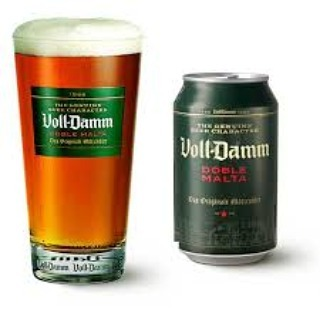
\includegraphics[width=0.9in, height=0.9in]{img/spam5} \label{fig:ob_inflamatory_histology}}
\subfloat{
\includegraphics[width=0.9in, height=0.9in]{img/spam6} \label{fig:ob_inflamatory_histology}}\\
\subfloat{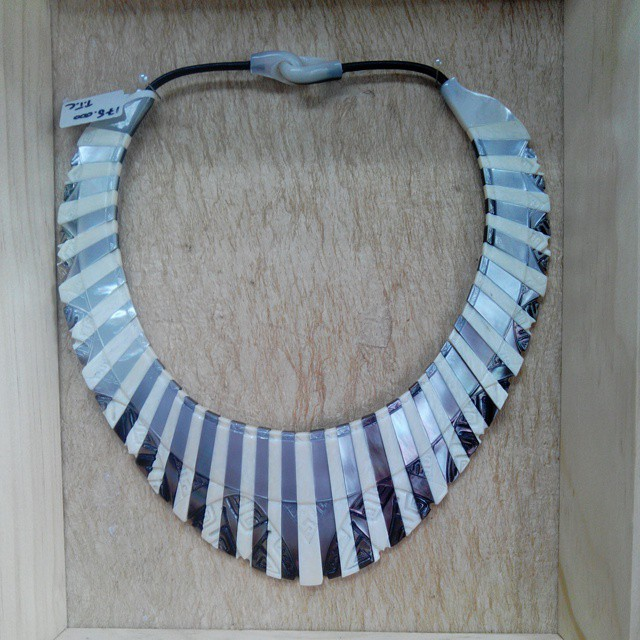
\includegraphics[width=0.9in, height=0.9in]{img/spam7} \label{fig:ob_inflamatory_histology}}
\subfloat{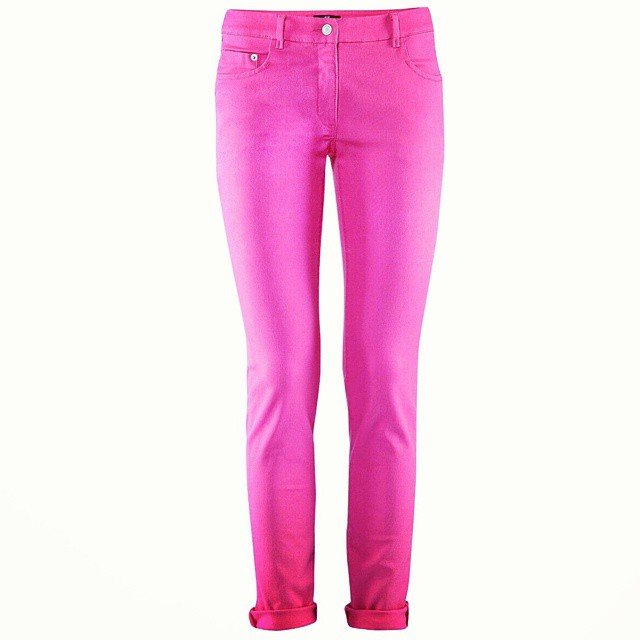
\includegraphics[width=0.9in, height=0.9in]{img/spam8} \label{fig:ob_inflamatory_histology}}
\subfloat{
\includegraphics[width=0.9in, height=0.9in]{img/spam9} \label{fig:ob_inflamatory_histology}}
\caption{Example true positives)}
\label{fig:spamexamples}
\end{figure}

\subsection{Deep convolutional networks based image classification on Instagram}

TODO (Leonel)

\subsection{Near-replica image detection on Twitter}

TODO (Dani Mora)

%
\section{Results}
%
The main goal of the experiments is to evaluate the speed-up, scale-up, and size-up properties of the proposed framework applied to the selected workloads. To this end, we use datasets up to hundreds of GBs TODO of raw data. The size of RDDs is reported to be 2-5 times larger than that; in our experiments 400GBs of data in the sort-by-key application correspond to an RDD of 1TB.
 The cluster sizes range from 8 cores up to 1024 (i.e., 64 machines)...TODO

We have submitted and tested several hundreds of jobs to MareNostrum, but we describe only the results that are of significance. Our runs include an extensive  set of configurations; for brevity, when those parameters were shown to be either irrelevant or to have negligible effect, we use default values. Each experimental configuration was repeated at least 5 times. Unless otherwise stated, we report median values in seconds. 

TODO (Ruben)

\subsection{Bag-of-Words based image classification on Instagram}

TODO (Mouna)

\subsubsection{speed-up} In the first set of experiments, we keep the input dataset constant and we increase the size of nodes/cores running the Spark application; whenever we refer to nodes, we mean  MareNostrum machines that run the executors, while the driver always runs on a separate machine; each machine is equipped with 16 cores and 32 GB of RAM. The results from 128 (8 nodes) up to 512 cores (32 nodes) are shown in Figure \ref{fig:speedup1}, where we can see that for large datasets in terms of number of records, the training can scale well. In the figure, we present the performance for the most efficient configurations; we discuss these configurations in detail later. TODO

\begin{figure}[tb!]
\begin{center}
\centerline{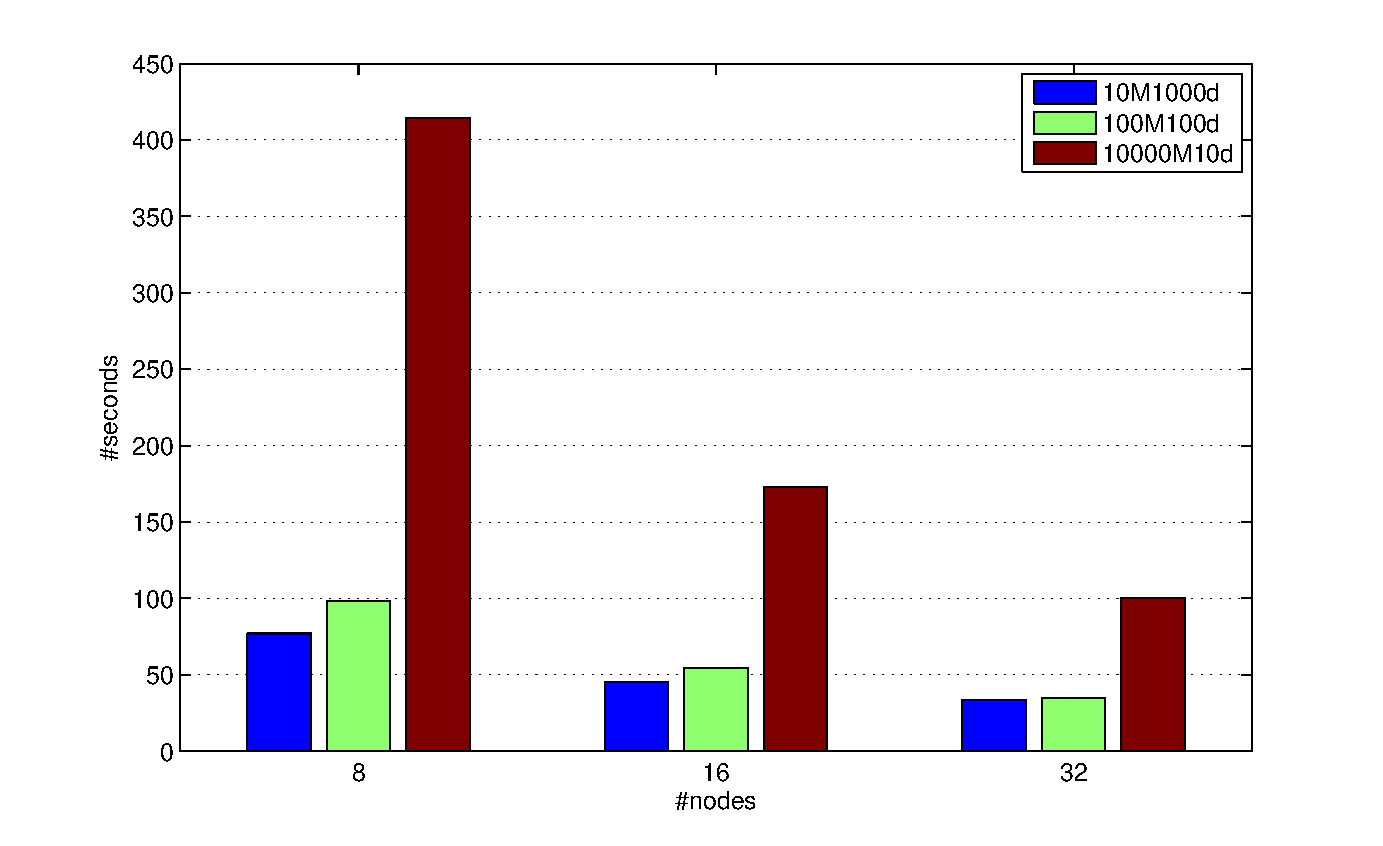
\includegraphics[width=0.75\linewidth]{img/speedup1.pdf}}
\caption{Times for training....}
\label{fig:speedup1}
\end{center}
\vspace{-0.5cm}
\end{figure}

\subsubsection{scale-up} We process the same datasets, and we now modify both the number of records and the number of machines, i.e., the infrastructure scales-out. .... The results are shown in Figure \ref{fig:scaleup1}(top). In this figure, we show both the average and the median values. Ideally, all the plots should be horizontal; our system behaves closely to that. ....

\begin{figure}[tb!]
\begin{center}
\centerline{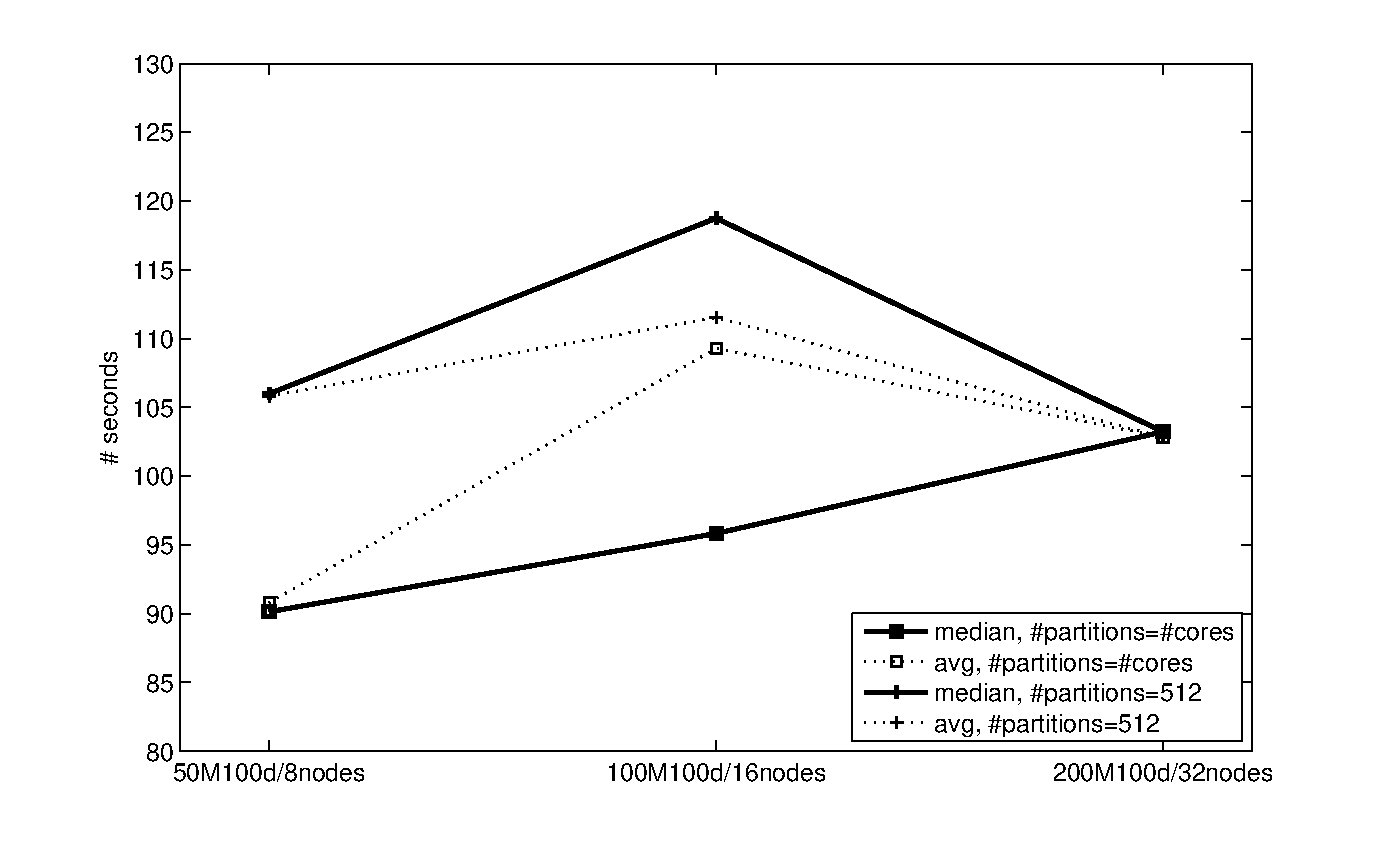
\includegraphics[width=0.75\linewidth]{img/scaleup1.pdf}}
\caption{Times for training....}
\label{fig:speedup1}
\end{center}
\vspace{-0.5cm}
\end{figure}

\subsubsection{size-up} We perform a third set of experiments, to assess the capability of sizing-up. We keep the number of nodes constant (either 16 or 32), and we gradually increase the dataset from 100GBs to 200GBs (raw data sizes). As shown in Figure \ref{fig:sizeup1}(bottom), Spark4MN exhibits a behavior where the curves are (almost) linear. ....

\begin{figure}[tb!]
\begin{center}
\centerline{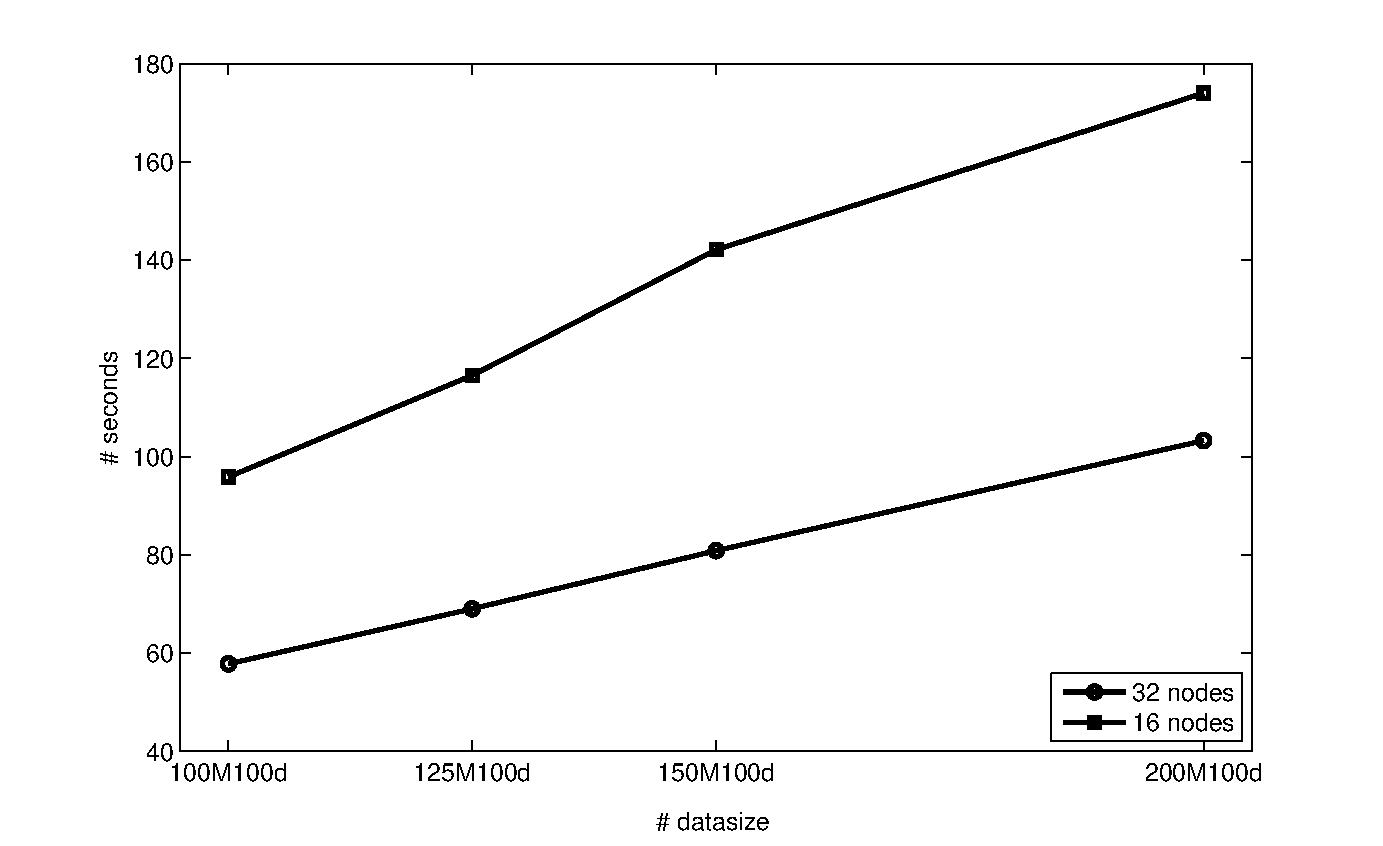
\includegraphics[width=0.75\linewidth]{img/sizeup1.pdf}}
\caption{Times for training....}
\label{fig:speedup1}
\end{center}
\vspace{-0.5cm}
\end{figure}

\subsection{Deep convolutional networks based image classification on Instagram}

TODO (Leonel)

\subsection{Near-replica image detection on Twitter}

TODO (Dani Mora)


%
\section{Conclusions}
%
The research work presented in this paper..... TODO

%%%%%%%%%%%%%%%%%%%%%%%%%%%%%%%%%%%%%%%%%%%
\section*{Acknowledgements}
%%%%%%%%%%%%%%%%%%%%%%%%%%%%%%%%%%%%%%%%%%%
This work is partially supported by the Spanish Ministry of Economy and Competitivity under contract TIN2015-65316-P and by the SGR programme (2014-SGR-1051) of the Catalan Government.

\begin{small}
\bibliographystyle{plain}
\bibliography{refs}
\end{small}

%\begin{IEEEbiography}[{\includegraphics[width=1in,height=1.25in,clip,keepaspectratio]{ruben_tous.jpg}}]{Ruben Tous}
%is an associate professor in the Department of Computer Architecture at Universitat Polit\`ecnica de Catalunya. BarcelonaTech (UPC). His scientific work focuses on algorithms and data structures, knowledge representation and reasoning for multimedia understanding, multimedia databases and query languages, and %multimedia information retrieval. Tous has a PhD in computer science and digital communications from Universitat Pompeu Fabra, Spain. Contact him at rtous@ac.upc.edu.
%\end{IEEEbiography}

%\begin{IEEEbiography}[{\includegraphics[width=1in,height=1.25in,clip,keepaspectratio]{jaime_delgado.jpg}}]{Jaime Delgado}
%is a professor in the Computer Architecture Department and the founder and head of the Distributed Multimedia Applications Group (DMAG) at Universitat Polit\`ecnica de Catalunya. BarcelonaTech (UPC). His research interests include multimedia applications, privacy, metadata interoperability, multimedia search and digital %management of rights. Delgado has a PhD in telecommunication engineering from UPC. Contact him at jaime.delgado@ac.upc.edu.
%\end{IEEEbiography}

\end{document}
